\subsection{Building your Deep Neural Network: Step by Step}

Welcome to your third programming exercise of the deep learning specialization. You will implement all the building blocks of a neural network and use these building blocks in the next assignment to build a neural network of any architecture you want. By completing this assignment you will:
\begin{itemize}
\item Develop an intuition of the over all structure of a neural network.

\item Write functions (e.g. forward propagation, backward propagation, logistic loss, etc...) that would help you decompose your code and ease the process of building a neural network.

\item Initialize/update parameters according to your desired structure.
\end{itemize}

This assignment prepares you well for the upcoming assignment. In the next assignment, you will use these functions to build a deep neural network for image classification. Take your time to complete it and make sure you get the expected outputs when working through the different exercises. In some code blocks, you will find a "\#GRADED FUNCTION: functionName" comment. Please do not modify it. After you are done, submit your work and check your results. You need to score 70\% to pass. Good luck :) !


After this assignment you will be able to:
\begin{itemize}
\item Use non-linear units like ReLU to improve your model
\item Build a deeper neural network (with more than 1 hidden layer)
\item Implement an easy-to-use neural network class
\end{itemize}


{\textbf {Notation}}:
\begin{itemize}
\item Superscript $[l]$ denotes a quantity associated with the $l^{th}$ layer. 
\begin{itemize}
\item Example: $a^{[L]}$ is the $L^{th}$ layer activation. $W^{[L]}$ and $b^{[L]}$ are the $L^{th}$ layer parameters.
\end{itemize}
\item Superscript $(i)$ denotes a quantity associated with the $i^{th}$ example. 
\begin{itemize}
\item Example: $x^{(i)}$ is the $i^{th}$ training example.
\end{itemize}
\item Lowerscript $i$ denotes the $i^{th}$ entry of a vector.
\begin{itemize}
\item Example: $a^{[l]}_i$ denotes the $i^{th}$ entry of the $l^{th}$ layer's activations).
\end{itemize}
\end{itemize}

Let's get started!


\subsubsection{Packages}

Let's first import all the packages that you will need during this assignment. 
\begin{itemize}
\item \href{www.numpy.org}{numpy} is the main package for scientific computing with Python.
\item \href{http://matplotlib.org}{matplotlib} is a library to plot graphs in Python.
\item dnn\_utils provides some necessary functions for this notebook.
\item testCases provides some test cases to assess the correctness of your functions
\item np.random.seed(1) is used to keep all the random function calls consistent. It will help us grade your work. Please don't change the seed. 
\end{itemize}

\subsubsection{Outline of the Assignment}

To build your neural network, you will be implementing several``helper functions". These helper functions will be used in the next assignment to build a two-layer neural network and an L-layer neural network. Each small helper function you will implement will have detailed instructions that will walk you through the necessary steps. Figure \ref{fig:final_outline} is an outline of this assignment, you will:

\begin{itemize}
\item Initialize the parameters for a two-layer network and for an $L$-layer neural network.
\item Implement the forward propagation module (shown in purple in the figure below).
     \begin{itemize}
     \item Complete the LINEAR part of a layer's forward propagation step (resulting in $Z^{[l]}$).
     \item We give you the ACTIVATION function (relu/sigmoid).
     \item Combine the previous two steps into a new [LINEAR->ACTIVATION] forward function.
     \item Stack the [LINEAR->RELU] forward function L-1 time (for layers 1 through L-1) and add a [LINEAR->SIGMOID] at the end (for the final layer $L$). This gives you a new L\_model\_forward function.
     \end{itemize}
\item Compute the loss.
\item Implement the backward propagation module (denoted in red in the figure below).
   \begin{itemize}
    \item Complete the LINEAR part of a layer's backward propagation step.
    \item We give you the gradient of the ACTIVATE function (relu\_backward/sigmoid\_backward) 
    \item Combine the previous two steps into a new [LINEAR->ACTIVATION] backward function.
    \item Stack [LINEAR->RELU] backward L-1 times and add [LINEAR->SIGMOID] backward in a new L\_model\_backward function
    \end{itemize}
\item Finally update the parameters.
\end{itemize}

\begin{figure}[h]
\begin{center}
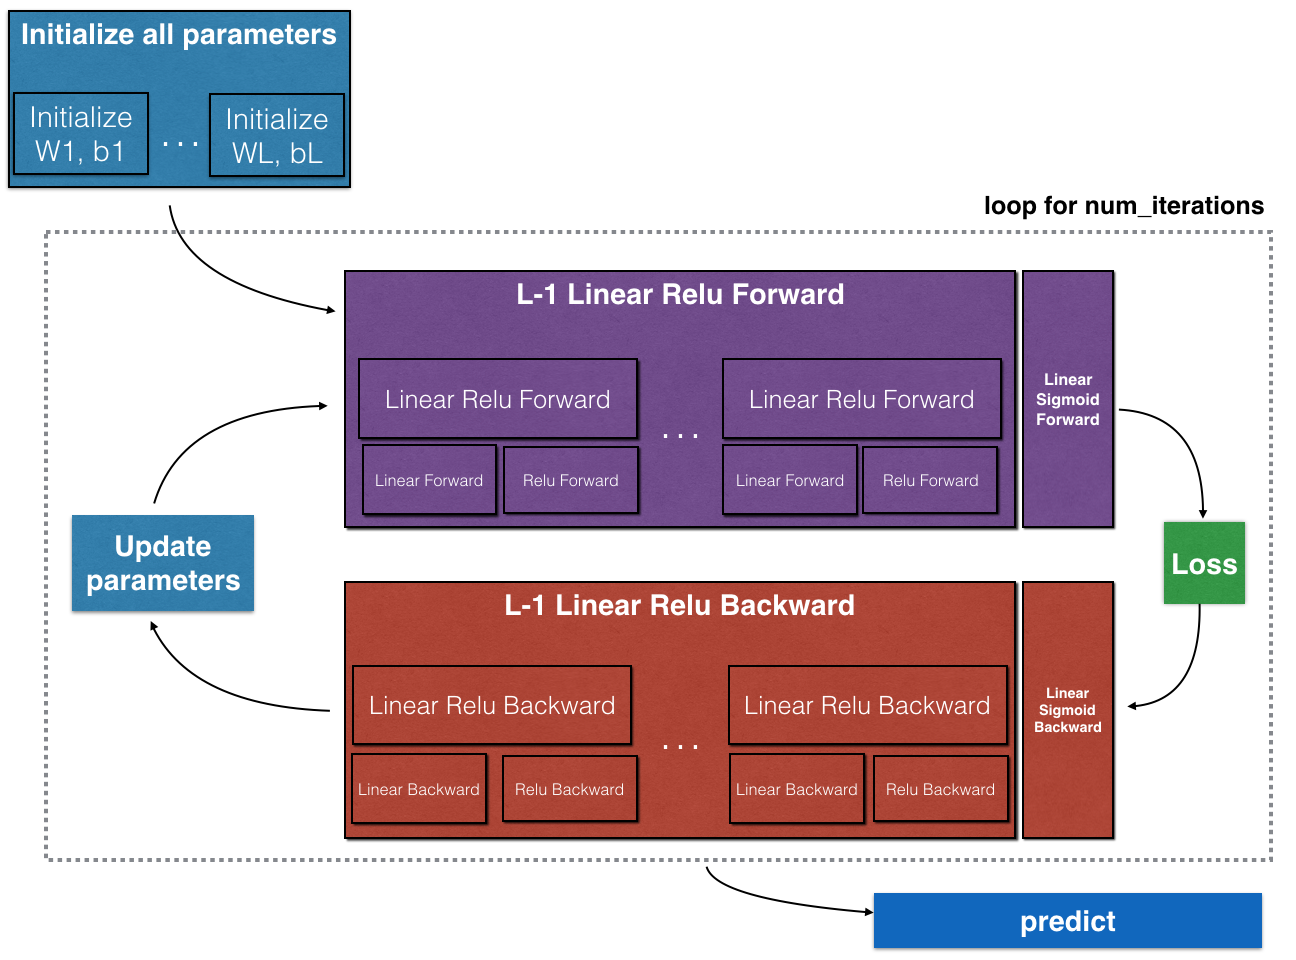
\includegraphics[width=0.5\textwidth]{course1/final_outline}
\end{center}
\caption{Outline}
\label{fig:final_outline}
\end{figure}

{\textbf {Note}} that for every forward function, there is a corresponding backward function. That is why at every step of your forward module you will be storing some values in a cache. The cached values are useful for computing gradients. In the backpropagation module you will then use the cache to calculate the gradients. This assignment will show you exactly how to carry out each of these steps.



\subsubsection{Initialization}

You will write two helper functions that will initialize the parameters for your model. The first function will be used to initialize parameters for a two layer model. The second one will generalize this initialization process to  $L$ layers.

\subsubsubsection{2-layer Neural Network}

{\textbf {Exercise}}: Create and initialize the parameters of the 2-layer neural network.

{\textbf {Instructions}}:
\begin{itemize}
\item The model's structure is: LINEAR -> RELU -> LINEAR -> SIGMOID.
\item Use random initialization for the weight matrices. Use np.random.randn(shape)*0.01 with the correct shape.
\item Use zero initialization for the biases. Use np.zeros(shape).
\end{itemize}

\begin{minted}{python}
# GRADED FUNCTION: initialize_parameters
def initialize_parameters(n_x, n_h, n_y):
    """
    Argument:
    n_x -- size of the input layer
    n_h -- size of the hidden layer
    n_y -- size of the output layer
    
    Returns:
    parameters -- python dictionary containing your parameters:
                    W1 -- weight matrix of shape (n_h, n_x)
                    b1 -- bias vector of shape (n_h, 1)
                    W2 -- weight matrix of shape (n_y, n_h)
                    b2 -- bias vector of shape (n_y, 1)
    """
    
    np.random.seed(1)
    
    ### START CODE HERE ### (≈ 4 lines of code)
    W1 = np.random.randn(n_h, n_x)*0.01
    b1 = np.zeros((n_h, 1))
    W2 = np.random.randn(n_y, n_h)*0.01
    b2 = np.zeros((n_y, 1))
    ### END CODE HERE ###
    
    assert(W1.shape == (n_h, n_x))
    assert(b1.shape == (n_h, 1))
    assert(W2.shape == (n_y, n_h))
    assert(b2.shape == (n_y, 1))
    
    parameters = {"W1": W1,
                  "b1": b1,
                  "W2": W2,
                  "b2": b2}
    
    return parameters
\end{minted}


\subsubsubsection{L-layer Neural Network}

The initialization for a deeper L-layer neural network is more complicated because there are many more weight matrices and bias vectors. When completing the ``initialize\_parameters\_deep'', you should make sure that your dimensions match between each layer. Recall that $n^{[l]}$ is the number of units in layer $l$. Thus for example if the size of our input $X$ is $(12288, 209)$ (with $m=209$ examples) then:


\begin{table}[H]
\centering
\begin{tabular}{ccccc}  
\toprule
 & Shape of W & Shape of b & Activation & Shape of Activation\\
\midrule
Layer 1 & $(n^{[1]},12288)$ & $(n^{[1]},1)$  & $Z^{[1]} = W^{[1]}  X + b^{[1]} $  & $(n^{[1]},209)$ \\
Layer 2 & $(n^{[2]}, n^{[1]})$ & $(n^{[2]},1)$  & $Z^{[2]} = W^{[2]} A^{[1]} + b^{[2]}$   & $(n^{[2]}, 209)$ \\
$\vdots$  & $\vdots$  & $\vdots$   & $\vdots$   & $\vdots$  \\
Layer L-1  & $(n^{[L-1]}, n^{[L-2]})$  & $(n^{[L-1]}, 1)$   & $Z^{[L-1]} =  W^{[L-1]} A^{[L-2]} + b^{[L-1]}$ & $(n^{[L-1]}, 209)$  \\
Layer L  & $(n^{[L]}, n^{[L-1]})$ & $(n^{[L]}, 1)$  & $Z^{[L]} =  W^{[L]} A^{[L-1]} + b^{[L]}$ & $(n^{[L]}, 209)$  \\
\bottomrule
\end{tabular}
\end{table}

Remember that when we compute $W X + b$ in python, it carries out broadcasting. For example, if: 
\begin{center}
$ W = \begin{bmatrix}
    j  & k  & l\\
    m  & n & o \\
    p  & q & r 
\end{bmatrix}\;\;\; X = \begin{bmatrix}
    a  & b  & c\\
    d  & e & f \\
    g  & h & i 
\end{bmatrix} \;\;\; b =\begin{bmatrix}
    s  \\
    t  \\
    u
\end{bmatrix}$
\end{center}

Then $WX + b$ will be:
\begin{equation}
WX + b = \begin{bmatrix}
    (ja + kd + lg) + s  & (jb + ke + lh) + s  & (jc + kf + li)+ s\\
    (ma + nd + og) + t & (mb + ne + oh) + t & (mc + nf + oi) + t\\
    (pa + qd + rg) + u & (pb + qe + rh) + u & (pc + qf + ri)+ u
\end{bmatrix}
\end{equation}


{\textbf {Exercise}}: Implement initialization for an L-layer Neural Network.

{\textbf {Instructions}}:
\begin{itemize}
\item The model's structure is [LINEAR -> RELU] $ \times$ (L-1) -> LINEAR -> SIGMOID. I.e., it has $L-1$ layers using a ReLU activation function followed by an output layer with a sigmoid activation function.
\item Use random initialization for the weight matrices. Use ``np.random.rand(shape) * 0.01''.
\item Use zeros initialization for the biases. Use ``np.zeros(shape)''.
\item We will store $n^{[l]}$, the number of units in different layers, in a variable ``layer\_dims''. For example, the ``layer\_dims'' for the ``Planar Data classification mode'' from last week would have been [2,4,1]: There were two inputs, one hidden layer with 4 hidden units, and an output layer with 1 output unit. Thus means ``W1'''s shape was (4,2), ``b1'' was (4,1), ``W2'' was (1,4) and ``b2'' was (1,1). Now you will generalize this to $L$ layers! 
\item Here is the implementation for $L=1$ (one layer neural network). It should inspire you to implement the general case (L-layer neural network).
\end{itemize}

\begin{mypython}
    if L == 1:
        parameters["W" + str(L)] = np.random.randn(layer_dims[1], layer_dims[0]) * 0.01
        parameters["b" + str(L)] = np.zeros((layer_dims[1], 1))
\end{mypython}




\begin{minted}{python}
# GRADED FUNCTION: initialize_parameters_deep
def initialize_parameters_deep(layer_dims):
    """
    Arguments:
    layer_dims -- python array (list) containing the dimensions of each layer in our network
    
    Returns:
    parameters -- python dictionary containing your parameters "W1", "b1", ..., "WL", "bL":
      Wl -- weight matrix of shape (layer_dims[l], layer_dims[l-1])
      bl -- bias vector of shape (layer_dims[l], 1)
    """
    
    np.random.seed(3)
    parameters = {}
    L = len(layer_dims)            # number of layers in the network

    for l in range(1, L):
        ### START CODE HERE ### (≈ 2 lines of code)
        parameters['W' + str(l)] = np.random.randn(layer_dims[l], layer_dims[l-1]) * 0.01
        parameters['b' + str(l)] = np.zeros((layer_dims[l], 1))
        ### END CODE HERE ###
        
        assert(parameters['W' + str(l)].shape == (layer_dims[l], layer_dims[l-1]))
        assert(parameters['b' + str(l)].shape == (layer_dims[l], 1))

        
    return parameters
\end{minted}



\subsubsection{Forward propagation module}
\subsubsubsection{Linear Forward}

Now that you have initialized your parameters, you will do the forward propagation module. You will start by implementing some basic functions that you will use later when implementing the model. You will complete three functions in this order:
\begin{itemize}
\item[1] LINEAR

\item[2] LINEAR -> ACTIVATION where ACTIVATION will be either ReLU or Sigmoid

\item[3] [LINEAR -> RELU] $\times$ (L-1) -> LINEAR -> SIGMOID (whole model)
\end{itemize}

The linear forward module (vectorized over all the examples) computes the following equations:
\begin{equation}
Z^{[l]} = W^{[l]}A^{[l-1]} +b^{[l]}
\end{equation}
where $A^{[0]} = X$. 

{\textbf {Exercise}}: Build the linear part of forward propagation.

{\textbf {Reminder}:
The mathematical representation of this unit is $Z^{[l]} = W^{[l]}A^{[l-1]} +b^{[l]}$. You may also find ``np.dot()'' useful. If your dimensions don't match, printing ``W.shape'' may help.

\begin{minted}{python}
# GRADED FUNCTION: linear_forward
def linear_forward(A, W, b):
    """
    Implement the linear part of a layer's forward propagation.

    Arguments:
    A -- activations from previous layer (or input data): (size of previous layer, number of examples)
    W -- weights matrix: numpy array of shape (size of current layer, size of previous layer)
    b -- bias vector, numpy array of shape (size of the current layer, 1)

    Returns:
    Z -- the input of the activation function, also called pre-activation parameter 
    cache -- a python dictionary containing "A", "W" and "b" ; stored for computing the backward pass efficiently
    """
    
    ### START CODE HERE ### (≈ 1 line of code)
    Z = np.dot(W,A)+b
    ### END CODE HERE ###
    
    assert(Z.shape == (W.shape[0], A.shape[1]))
    cache = (A, W, b)
    
    return Z, cache
\end{minted}    
    

\subsubsubsection{Linear-Activation Forward }

In this notebook, you will use two activation functions:

{\textbf {Sigmoid}}: $\sigma(Z) = \sigma(W A + b) = \frac{1}{ 1 + e^{-(W A + b)}}$. We have provided you with the ``sigmoid'' function. This function returns {\textbf {two}} items: the activation value ``a'' and a ``cache'' that contains ``Z'' (it's what we will feed in to the corresponding backward function). To use it you could just call: 
\begin{mypython}  
A, activation_cache = sigmoid(Z)
\end{mypython}  

{\textbf {ReLU}}: The mathematical formula for ReLu is $A = RELU(Z) = max(0, Z)$. We have provided you with the ``relu'' function. This function returns {\textbf {two}} items: the activation value ``A'' and a ``cache'' that contains ``Z'' (it's what we will feed in to the corresponding backward function). To use it you could just call:
\begin{mypython}  
A, activation_cache = relu(Z)
\end{mypython}  
 
For more convenience, you are going to group two functions (Linear and Activation) into one function (LINEAR->ACTIVATION). Hence, you will implement a function that does the LINEAR forward step followed by an ACTIVATION forward step.

{\textbf {Exercise}}: Implement the forward propagation of the \emph{LINEAR->ACTIVATION} layer. Mathematical relation is: $A^{[l]} = g(Z^{[l]}) = g(W^{[l]}A^{[l-1]} +b^{[l]})$ where the activation ``g'' can be sigmoid() or relu(). Use linear\_forward() and the correct activation function.


\begin{minted}{python} 
# GRADED FUNCTION: linear_activation_forward
def linear_activation_forward(A_prev, W, b, activation):
    """
    Implement the forward propagation for the LINEAR->ACTIVATION layer

    Arguments:
    A_prev -- activations from previous layer (or input data): (size of previous layer, number of examples)
    W -- weights matrix: numpy array of shape (size of current layer, size of previous layer)
    b -- bias vector, numpy array of shape (size of the current layer, 1)
    activation -- the activation to be used in this layer, stored as a text string: "sigmoid" or "relu"

    Returns:
    A -- the output of the activation function, also called the post-activation value 
    cache -- a python dictionary containing "linear_cache" and "activation_cache";
             stored for computing the backward pass efficiently
    """
    
    if activation == "sigmoid":
        # Inputs: "A_prev, W, b". Outputs: "A, activation_cache".
        ### START CODE HERE ### (≈ 2 lines of code)
        Z, linear_cache = linear_forward(A_prev, W, b)
        A, activation_cache = sigmoid(Z)
        ### END CODE HERE ###
    
    elif activation == "relu":
        # Inputs: "A_prev, W, b". Outputs: "A, activation_cache".
        ### START CODE HERE ### (≈ 2 lines of code)
        Z, linear_cache = linear_forward(A_prev, W, b)
        A, activation_cache = relu(Z)
        ### END CODE HERE ###
    
    assert (A.shape == (W.shape[0], A_prev.shape[1]))
    cache = (linear_cache, activation_cache)

    return A, cache
\end{minted}  

{\textbf {Note}}: In deep learning, the \emph{[LINEAR->ACTIVATION]} computation is counted as a single layer in the neural network, not two layers.    


\subsubsubsection{L-Layer Model}

For even more convenience when implementing the $L$-layer Neural Net, you will need a function that replicates the previous one (linear\_activation\_forward with RELU) $L-1$ times, then follows that with one linear\_activation\_forward with SIGMOID.

\begin{figure}[h]
\begin{center}
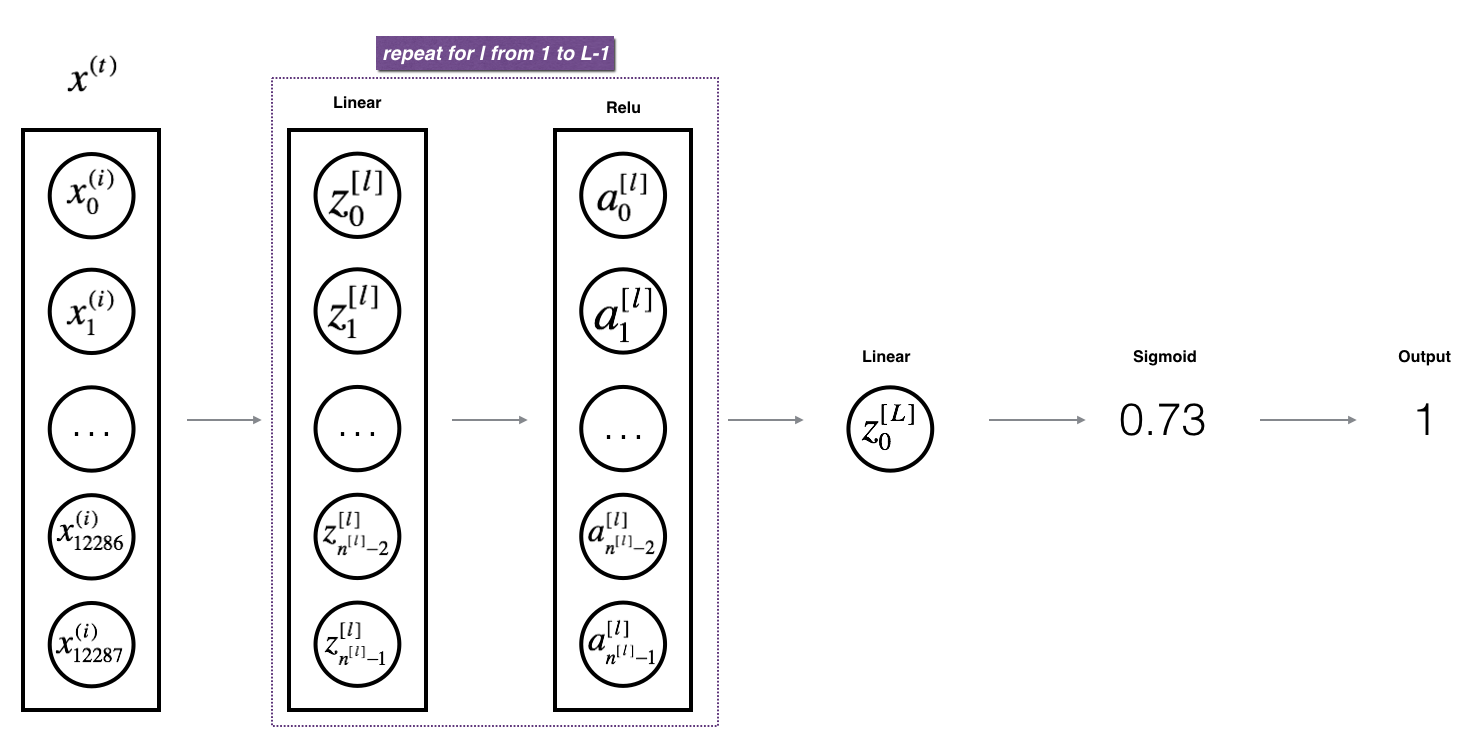
\includegraphics[width=\textwidth]{course1/model_architecture}
\end{center}
\caption{[LINEAR -> RELU] $\times$ (L-1) -> LINEAR -> SIGMOID model}
\label{fig:final_outline}
\end{figure}

{\textbf {Exercise}}: Implement the forward propagation of the above model.

{\textbf {Instruction}}: In the code below, the variable ``AL'' will denote $A^{[L]} = \sigma(Z^{[L]}) = \sigma(W^{[L]} A^{[L-1]} + b^{[L]})$. (This is sometimes also called ``Yhat'', i.e., this is $\hat{Y}$.) 

{\textbf {Tips}}:
\begin{itemize}
\item Use the functions you had previously written 
\item Use a for loop to replicate [LINEAR->RELU] (L-1) times
\item Don't forget to keep track of the caches in the ``caches'' list. To add a new value ``c'' to a ``list'', you can use ``list.append(c)''.
\end{itemize}

\begin{minted}{python}
# GRADED FUNCTION: L_model_forward
def L_model_forward(X, parameters):
    """
    Implement forward propagation for the [LINEAR->RELU]*(L-1)->LINEAR->SIGMOID computation
    
    Arguments:
    X -- data, numpy array of shape (input size, number of examples)
    parameters -- output of initialize_parameters_deep()
    
    Returns:
    AL -- last post-activation value
    caches -- list of caches containing:
                every cache of linear_relu_forward() (there are L-1 of them, indexed from 0 to L-2)
                the cache of linear_sigmoid_forward() (there is one, indexed L-1)
    """

    caches = []
    A = X
    L = len(parameters) // 2 # number of layers in the neural network
    
    # Implement [LINEAR -> RELU]*(L-1). Add "cache" to the "caches" list.
    for l in range(1, L):
        A_prev = A 
        ### START CODE HERE ### (≈ 2 lines of code)
        A, cache = linear_activation_forward(A_prev, parameters['W' + str(l)], parameters['b' + str(l)], activation ="relu")
        caches.append(cache)
        ### END CODE HERE ###
    
    # Implement LINEAR -> SIGMOID. Add "cache" to the "caches" list.
    ### START CODE HERE ### (≈ 2 lines of code)
    AL, cache = linear_activation_forward(A, parameters['W' + str(L)], parameters['b' + str(L)], activation = "sigmoid")
    caches.append(cache)
    ### END CODE HERE ###
    
    assert(AL.shape == (1,X.shape[1]))
            
    return AL, caches
\end{minted}

Great! Now you have a full forward propagation that takes the input X and outputs a row vector $A^{[L]}$ containing your predictions. It also records all intermediate values in ``caches''. Using $A^{[L]}$, you can compute the cost of your predictions.




\subsubsection{Cost function}

Now you will implement forward and backward propagation. You need to compute the cost, because you want to check if your model is actually learning.

{\textbf {Exercise}}: Compute the cross-entropy cost $J$, using the following formula: 
\begin{equation}
\frac{1}{m} \sum\limits_{i = 1}^{m} (y^{(i)}\log\left(a^{[L] (i)}\right) + (1-y^{(i)})\log\left(1- a^{[L](i)}\right)) 
\end{equation}

\begin{minted}{python}
# GRADED FUNCTION: compute_cost
def compute_cost(AL, Y):
    """
    Implement the cost function defined by equation (7).

    Arguments:
    AL -- probability vector corresponding to your label predictions, shape (1, number of examples)
    Y -- true "label" vector (for example: containing 0 if non-cat, 1 if cat), shape (1, number of examples)

    Returns:
    cost -- cross-entropy cost
    """
    
    m = Y.shape[1]

    # Compute loss from aL and y.
    ### START CODE HERE ### (≈ 1 lines of code)
    cost = -(np.dot(Y,np.log(AL.T))+np.dot(1-Y,np.log(1-AL).T))/m
    ### END CODE HERE ###
    
    cost = np.squeeze(cost)      # To make sure your cost's shape is what we expect (e.g. this turns [[17]] into 17).
    assert(cost.shape == ())
    
    return cost
\end{minted}


\subsubsection{Backward propagation module}

Just like with forward propagation, you will implement helper functions for backpropagation. Remember that back propagation is used to calculate the gradient of the loss function with respect to the parameters.

{\textbf {Reminder}}:

\begin{figure}[h]
\begin{center}
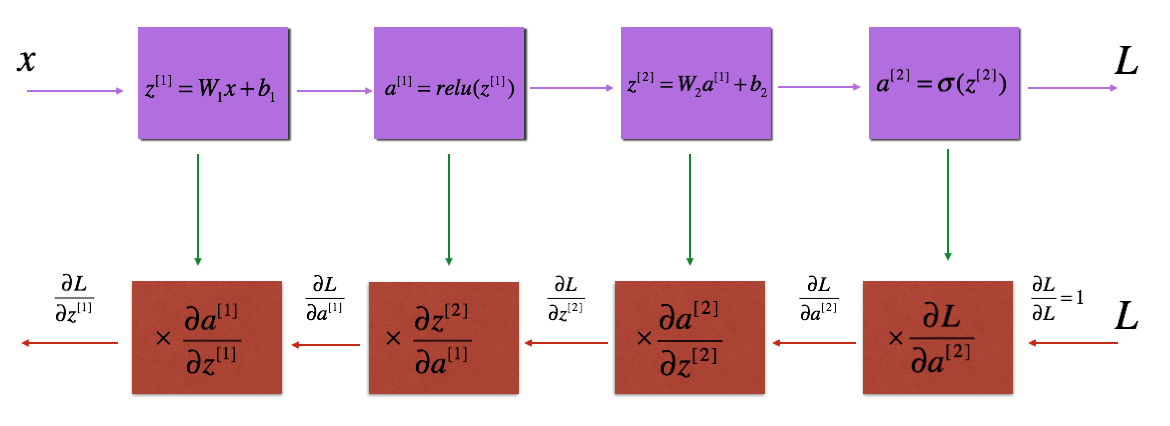
\includegraphics[width=\textwidth]{course1/backprop}
\end{center}
\caption{ Forward and Backward propagation for LINEAR->RELU->LINEAR->SIGMOID. The purple blocks represent the forward propagation, and the red blocks represent the backward propagation.}
\label{fig:backprop}
\end{figure}

Now, similar to forward propagation, you are going to build the backward propagation in three steps:
\begin{itemize}
\item[1] LINEAR backward
\item[2] LINEAR -> ACTIVATION backward where ACTIVATION computes the derivative of either the ReLU or sigmoid activation
\item[3] [LINEAR -> RELU] $\times $ (L-1) -> LINEAR -> SIGMOID backward (whole model)
\end{itemize}



\subsubsubsection{Linear backward}

\begin{figure}[h]
\begin{center}
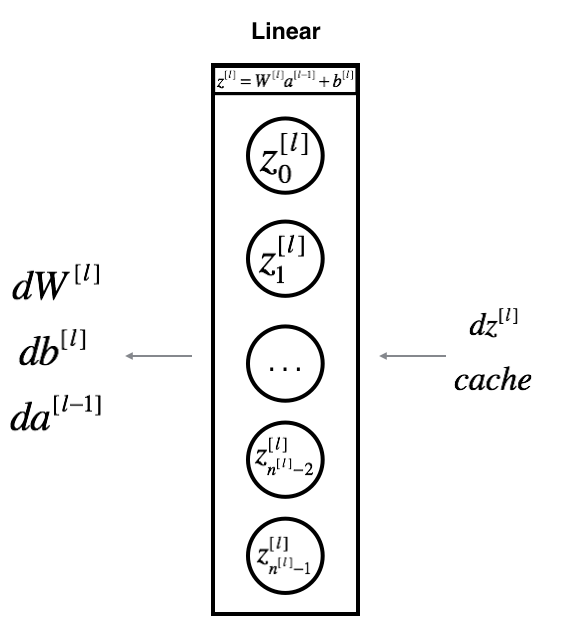
\includegraphics[width=0.34\textwidth]{course1/linearback}
\end{center}
\caption{Linear backward}
\label{fig:linearback}
\end{figure}

For layer $l$, the linear part is: $Z^{[l]} = W^{[l]} A^{[l-1]} + b^{[l]}$ (followed by an activation).

Suppose you have already calculated the derivative $dZ^{[l]} = \frac{\partial \mathcal{L} }{\partial Z^{[l]}}$. You want to get $(dW^{[l]}, db^{[l]} dA^{[l-1]})$.

The three outputs $(dW^{[l]}, db^{[l]}, dA^{[l]})$ are computed using the input $dZ^{[l]}$.Here are the formulas you need:
\begin{align}
dW^{[l]} = \frac{\partial \mathcal{L} }{\partial W^{[l]}} &= \frac{1}{m} dZ^{[l]} A^{[l-1] T} \\
db^{[l]} = \frac{\partial \mathcal{L} }{\partial b^{[l]}} &= \frac{1}{m} \sum_{i = 1}^{m} dZ^{[l](i)}\\
dA^{[l-1]} = \frac{\partial \mathcal{L} }{\partial A^{[l-1]}} &= W^{[l] T} dZ^{[l]} 
\end{align}

{\textbf {Exercise:}} Use the 3 formulas above to implement linear\_backward().

\begin{minted}{python}
# GRADED FUNCTION: linear_backward

def linear_backward(dZ, cache):
    """
    Implement the linear portion of backward propagation for a single layer (layer l)

    Arguments:
    dZ -- Gradient of the cost with respect to the linear output (of current layer l)
    cache -- tuple of values (A_prev, W, b) coming from the forward propagation in the current layer

    Returns:
    dA_prev -- Gradient of the cost with respect to the activation (of the previous layer l-1), same shape as A_prev
    dW -- Gradient of the cost with respect to W (current layer l), same shape as W
    db -- Gradient of the cost with respect to b (current layer l), same shape as b
    """
    A_prev, W, b = cache
    m = A_prev.shape[1]

    ### START CODE HERE ### (≈ 3 lines of code)
    dW = np.dot(dZ,A_prev.T)/m
    db = np.sum(dZ,axis=1,keepdims=True)/m
    dA_prev = np.dot(W.T,dZ)
    ### END CODE HERE ###
    
    assert (dA_prev.shape == A_prev.shape)
    assert (dW.shape == W.shape)
    assert (db.shape == b.shape)
    
    return dA_prev, dW, db
\end{minted}



\subsubsubsection{Linear-Activation backward}

Next, you will create a function that merges the two helper functions: {\textbf {linear\_backward}} and the backward step for the activation {\textbf {linear\_activation\_backward}}. 

To help you implement \emph{linear\_activation\_backward}, we provided two backward functions:
\begin{itemize}
\item {\textbf {sigmoid\_backward}}: Implements the backward propagation for SIGMOID unit. You can call it as follows:
\begin{minted}{python}
dZ = sigmoid_backward(dA, activation_cache)
\end{minted}
\item {\textbf {relu\_backward}}: Implements the backward propagation for RELU unit. You can call it as follows:
\begin{minted}{python}
dZ = relu_backward(dA, activation_cache)
\end{minted}
\end{itemize}

If $g(.)$ is the activation function, \emph{sigmoid\_backward} and \emph{relu\_backward} compute 
\begin{equation}
dZ^{[l]} = dA^{[l]} * g'(Z^{[l]})
\end{equation}

{\textbf {Exercise}}: Implement the backpropagation for the \emph{LINEAR->ACTIVATION} layer.

\begin{minted}{python}
# GRADED FUNCTION: linear_activation_backward
def linear_activation_backward(dA, cache, activation):
    """
    Implement the backward propagation for the LINEAR->ACTIVATION layer.
    
    Arguments:
    dA -- post-activation gradient for current layer l 
    cache -- tuple of values (linear_cache, activation_cache) we store for computing backward propagation efficiently
    activation -- the activation to be used in this layer, stored as a text string: "sigmoid" or "relu"
    
    Returns:
    dA_prev -- Gradient of the cost with respect to the activation (of the previous layer l-1), same shape as A_prev
    dW -- Gradient of the cost with respect to W (current layer l), same shape as W
    db -- Gradient of the cost with respect to b (current layer l), same shape as b
    """
    linear_cache, activation_cache = cache
    
    if activation == "relu":
        ### START CODE HERE ### (≈ 2 lines of code)
        dZ =  relu_backward(dA, activation_cache)
        dA_prev, dW, db = linear_backward(dZ, linear_cache)
        ### END CODE HERE ###
        
    elif activation == "sigmoid":
        ### START CODE HERE ### (≈ 2 lines of code)
        dZ =  sigmoid_backward(dA, activation_cache)
        dA_prev, dW, db = linear_backward(dZ, linear_cache)
        ### END CODE HERE ###
    
    return dA_prev, dW, db
\end{minted}


\subsubsubsection{L-Model Backward}

Now you will implement the backward function for the whole network. Recall that when you implemented the \emph{L\_model\_forward} function, at each iteration, you stored a cache which contains (X,W,b, and z). In the back propagation module, you will use those variables to compute the gradients. Therefore, in the \emph{L\_model\_backward} function, you will iterate through all the hidden layers backward, starting from layer $L$. On each step, you will use the cached values for layer $l$ to backpropagate through layer $l$. Figure \ref{fig: backward} below shows the backward pass. 

\begin{figure}[h]
\begin{center}
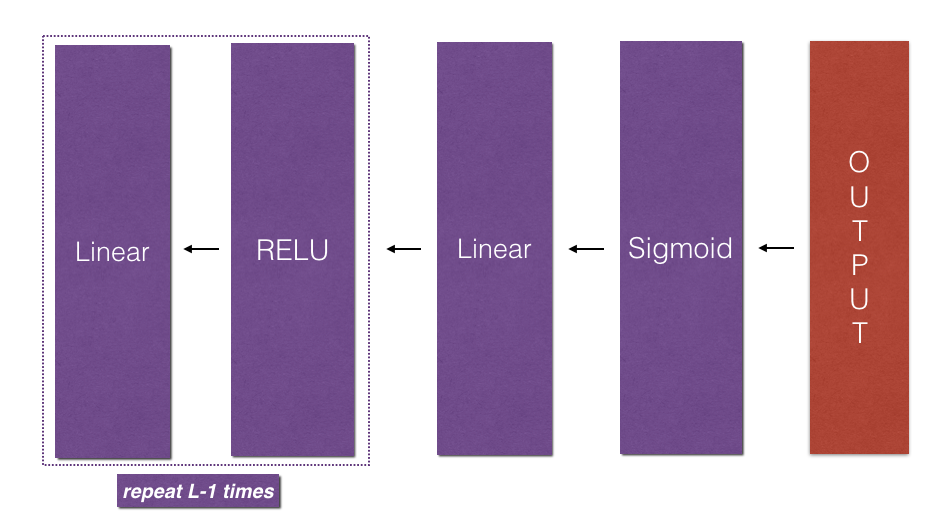
\includegraphics[width=0.8\textwidth]{course1/backward}
\end{center}
\caption{Backward pass}
\label{fig: backward}
\end{figure}


{\textbf {Initializing backpropagation}}:
To backpropagate through this network, we know that the output is, 
$A^{[L]} = \sigma(Z^{[L]})$. Your code thus needs to compute \emph{dAL} $= \frac{\partial \mathcal{L}}{\partial A^{[L]}}$.
To do so, use this formula (derived using calculus which you don't need in-depth knowledge of):
\begin{minted}{python}
dAL = - (np.divide(Y, AL) - np.divide(1 - Y, 1 - AL)) # derivative of cost with respect to AL
\end{minted}

You can then use this post-activation gradient \emph{dAL} to keep going backward. As seen in Figure \ref{fig: backward}, you can now feed in \emph{dAL} into the LINEAR->SIGMOID backward function you implemented (which will use the cached values stored by the L\_model\_forward function). After that, you will have to use a \emph{for} loop to iterate through all the other layers using the LINEAR->RELU backward function. You should store each dA, dW, and db in the grads dictionary. To do so, use this formula : 
\begin{equation}
grads[``dW" + str(l)] = dW^{[l]}
\end{equation}

For example, for $l=3$ this would store $dW^{[l]}$ in \emph{grads[``dW3"]}.

{\textbf {Exercise}}: Implement backpropagation for the \emph{[LINEAR->RELU] $\times$ (L-1) -> LINEAR -> SIGMOID} model.

\begin{minted}{python}
# GRADED FUNCTION: L_model_backward
def L_model_backward(AL, Y, caches):
    """
    Implement the backward propagation for the [LINEAR->RELU] * (L-1) -> LINEAR -> SIGMOID group
    
    Arguments:
    AL -- probability vector, output of the forward propagation (L_model_forward())
    Y -- true "label" vector (containing 0 if non-cat, 1 if cat)
    caches -- list of caches containing:
                every cache of linear_activation_forward() with "relu" (it's caches[l], for l in range(L-1) i.e l = 0...L-2)
                the cache of linear_activation_forward() with "sigmoid" (it's caches[L-1])
    
    Returns:
    grads -- A dictionary with the gradients
             grads["dA" + str(l)] = ... 
             grads["dW" + str(l)] = ...
             grads["db" + str(l)] = ... 
    """
    grads = {}
    L = len(caches) # the number of layers
    m = AL.shape[1]
    Y = Y.reshape(AL.shape) # after this line, Y is the same shape as AL
    
    # Initializing the backpropagation
    ### START CODE HERE ### (1 line of code)
    dAL =  - (np.divide(Y, AL) - np.divide(1 - Y, 1 - AL))
    ### END CODE HERE ###
    
    # Lth layer (SIGMOID -> LINEAR) gradients. Inputs: "AL, Y, caches". Outputs: "grads["dAL"], grads["dWL"], grads["dbL"]
    ### START CODE HERE ### (approx. 2 lines)
    current_cache = caches[L-1]
    grads["dA" + str(L)], grads["dW" + str(L)], grads["db" + str(L)] =  linear_activation_backward(dAL, current_cache, "sigmoid")
    ### END CODE HERE ###
    
    for l in reversed(range(L-1)):
        # lth layer: (RELU -> LINEAR) gradients.
        # Inputs: "grads["dA" + str(l + 2)], caches". Outputs: "grads["dA" + str(l + 1)] , grads["dW" + str(l + 1)] , grads["db" + str(l + 1)] 
        ### START CODE HERE ### (approx. 5 lines)
        current_cache = caches[l]
        dA_prev_temp, dW_temp, db_temp = linear_activation_backward(grads["dA" + str(l+2)], current_cache, "relu")
        grads["dA" + str(l + 1)] = dA_prev_temp
        grads["dW" + str(l + 1)] = dW_temp
        grads["db" + str(l + 1)] = db_temp
        ### END CODE HERE ###

    return grads
\end{minted}


\subsubsubsection{Update Parameters}

In this section you will update the parameters of the model, using gradient descent: 
\begin{align}
W^{[l]} &= W^{[l]} - \alpha \text{ } dW^{[l]} \\
b^{[l]} &= b^{[l]} - \alpha \text{ } db^{[l]}
\end{align}
where $\alpha$ is the learning rate. After computing the updated parameters, store them in the parameters dictionary. 

{\textbf {Exercise}}: Implement ``update\_parameters()'' to update your parameters using gradient descent.

{\textbf {Instructions}}:
Update parameters using gradient descent on every $W^{[l]}$ and $b^{[l]}$ for $l = 1, 2, ..., L$. 
\begin{minted}{python}
# GRADED FUNCTION: update_parameters
def update_parameters(parameters, grads, learning_rate):
    """
    Update parameters using gradient descent
    
    Arguments:
    parameters -- python dictionary containing your parameters 
    grads -- python dictionary containing your gradients, output of L_model_backward
    
    Returns:
    parameters -- python dictionary containing your updated parameters 
                  parameters["W" + str(l)] = ... 
                  parameters["b" + str(l)] = ...
    """
    
    L = len(parameters) // 2 # number of layers in the neural network

    # Update rule for each parameter. Use a for loop.
    ### START CODE HERE ### (≈ 3 lines of code)
    for l in range(L):
        parameters["W" + str(l+1)] =  parameters["W" + str(l+1)] - learning_rate * grads["dW" + str(l + 1)]
        parameters["b" + str(l+1)] = parameters["b" + str(l+1)] - learning_rate * grads["db" + str(l + 1)]
    ### END CODE HERE ###
    return parameters
\end{minted}




\subsubsubsection{Conclusion}

Congrats on implementing all the functions required for building a deep neural network!

We know it was a long assignment but going forward it will only get better. The next part of the assignment is easier.

In the next assignment you will put all these together to build two models:
\begin{itemize}
\item A two-layer neural network
\item An L-layer neural network
\end{itemize}

You will in fact use these models to classify cat vs non-cat images!



\clearpage
\subsubsection{Code of Deep Neural Network}
\begin{minted}{python}
import numpy as np
import h5py
import matplotlib.pyplot as plt
from testCases_v3 import *
from dnn_utils_v2 import sigmoid, sigmoid_backward, relu, relu_backward

#matplotlib inline
plt.rcParams['figure.figsize'] = (5.0, 4.0) # set default size of plots
plt.rcParams['image.interpolation'] = 'nearest'
plt.rcParams['image.cmap'] = 'gray'


# GRADED FUNCTION: initialize_parameters
def initialize_parameters(n_x, n_h, n_y):
    """
    Argument:
    n_x -- size of the input layer
    n_h -- size of the hidden layer
    n_y -- size of the output layer
    
    Returns:
    parameters -- python dictionary containing your parameters:
                    W1 -- weight matrix of shape (n_h, n_x)
                    b1 -- bias vector of shape (n_h, 1)
                    W2 -- weight matrix of shape (n_y, n_h)
                    b2 -- bias vector of shape (n_y, 1)
    """
    
    np.random.seed(1)
    
    W1 = np.random.randn(n_h, n_x)*0.01
    b1 = np.zeros((n_h, 1))
    W2 = np.random.randn(n_y, n_h)*0.01
    b2 = np.zeros((n_y, 1))
    
    assert(W1.shape == (n_h, n_x))
    assert(b1.shape == (n_h, 1))
    assert(W2.shape == (n_y, n_h))
    assert(b2.shape == (n_y, 1))
    
    parameters = {"W1": W1,
                  "b1": b1,
                  "W2": W2,
                  "b2": b2}
    
    return parameters


# GRADED FUNCTION: initialize_parameters_deep
def initialize_parameters_deep(layer_dims):
    """
    Arguments:
    layer_dims -- python array (list) containing the dimensions of each layer in our network
    
    Returns:
    parameters -- python dictionary containing your parameters "W1", "b1", ..., "WL", "bL":
                    Wl -- weight matrix of shape (layer_dims[l], layer_dims[l-1])
                    bl -- bias vector of shape (layer_dims[l], 1)
    """
    
    np.random.seed(3)
    parameters = {}
    L = len(layer_dims)            # number of layers in the network

    for l in range(1, L):
        parameters['W' + str(l)] = np.random.randn(layer_dims[l], layer_dims[l-1]) * 0.01
        parameters['b' + str(l)] = np.zeros((layer_dims[l], 1))
        
        assert(parameters['W' + str(l)].shape == (layer_dims[l], layer_dims[l-1]))
        assert(parameters['b' + str(l)].shape == (layer_dims[l], 1))
       
    return parameters


# GRADED FUNCTION: linear_forward
def linear_forward(A, W, b):
    """
    Implement the linear part of a layer's forward propagation.

    Arguments:
    A -- activations from previous layer (or input data): (size of previous layer, number of examples)
    W -- weights matrix: numpy array of shape (size of current layer, size of previous layer)
    b -- bias vector, numpy array of shape (size of the current layer, 1)

    Returns:
    Z -- the input of the activation function, also called pre-activation parameter 
    cache -- a python dictionary containing "A", "W" and "b" ; stored for computing the backward pass efficiently
    """
    
    Z = np.dot(W,A)+b
    
    assert(Z.shape == (W.shape[0], A.shape[1]))
    cache = (A, W, b)
    
    return Z, cache


def linear_activation_forward(A_prev, W, b, activation):
    """
    Implement the forward propagation for the LINEAR->ACTIVATION layer

    Arguments:
    A_prev -- activations from previous layer (or input data): (size of previous layer, number of examples)
    W -- weights matrix: numpy array of shape (size of current layer, size of previous layer)
    b -- bias vector, numpy array of shape (size of the current layer, 1)
    activation -- the activation to be used in this layer, stored as a text string: "sigmoid" or "relu"

    Returns:
    A -- the output of the activation function, also called the post-activation value 
    cache -- a python dictionary containing "linear_cache" and "activation_cache";
             stored for computing the backward pass efficiently
    """
    
    if activation == "sigmoid":
        # Inputs: "A_prev, W, b". Outputs: "A, activation_cache".
        Z, linear_cache = linear_forward(A_prev, W, b)
        A, activation_cache = sigmoid(Z)
    
    elif activation == "relu":
        # Inputs: "A_prev, W, b". Outputs: "A, activation_cache".
        Z, linear_cache = linear_forward(A_prev, W, b)
        A, activation_cache = relu(Z)
    
    assert (A.shape == (W.shape[0], A_prev.shape[1]))
    cache = (linear_cache, activation_cache)

    return A, cache


# GRADED FUNCTION: L_model_forward
def L_model_forward(X, parameters):
    """
    Implement forward propagation for the [LINEAR->RELU]*(L-1)->LINEAR->SIGMOID computation
    
    Arguments:
    X -- data, numpy array of shape (input size, number of examples)
    parameters -- output of initialize_parameters_deep()
    
    Returns:
    AL -- last post-activation value
    caches -- list of caches containing:
                every cache of linear_relu_forward() (there are L-1 of them, indexed from 0 to L-2)
                the cache of linear_sigmoid_forward() (there is one, indexed L-1)
    """

    caches = []
    A = X
    L = len(parameters) // 2     # number of layers in the neural network
    
    # Implement [LINEAR -> RELU]*(L-1). Add "cache" to the "caches" list.
    for l in range(1, L):
        A_prev = A 
        A, cache = linear_activation_forward(A_prev, parameters['W' + str(l)], parameters['b' + str(l)], activation ="relu")
        caches.append(cache)
    
    # Implement LINEAR -> SIGMOID. Add "cache" to the "caches" list.
    AL, cache = linear_activation_forward(A, parameters['W' + str(L)], parameters['b' + str(L)], activation = "sigmoid")
    caches.append(cache)
    
    assert(AL.shape == (1,X.shape[1]))
            
    return AL, caches


# GRADED FUNCTION: compute_cost
def compute_cost(AL, Y):
    """
    Implement the cost function defined by equation (7).

    Arguments:
    AL -- probability vector corresponding to your label predictions, shape (1, number of examples)
    Y -- true "label" vector (for example: containing 0 if non-cat, 1 if cat), shape (1, number of examples)

    Returns:
    cost -- cross-entropy cost
    """
    
    m = Y.shape[1]
    # Compute loss from aL and y.
    cost = -(np.dot(Y,np.log(AL.T))+np.dot(1-Y,np.log(1-AL).T))/m
    
    cost = np.squeeze(cost)      # To make sure your cost's shape is what we expect (e.g. this turns [[17]] into 17).
    assert(cost.shape == ())
    
    return cost


# GRADED FUNCTION: linear_backward
def linear_backward(dZ, cache):
    """
    Implement the linear portion of backward propagation for a single layer (layer l)

    Arguments:
    dZ -- Gradient of the cost with respect to the linear output (of current layer l)
    cache -- tuple of values (A_prev, W, b) coming from the forward propagation in the current layer

    Returns:
    dA_prev -- Gradient of the cost with respect to the activation (of the previous layer l-1), same shape as A_prev
    dW -- Gradient of the cost with respect to W (current layer l), same shape as W
    db -- Gradient of the cost with respect to b (current layer l), same shape as b
    """
    A_prev, W, b = cache
    m = A_prev.shape[1]

    dW = np.dot(dZ,A_prev.T)/m
    db = np.sum(dZ,axis=1,keepdims=True)/m
    dA_prev = np.dot(W.T,dZ)
    
    assert (dA_prev.shape == A_prev.shape)
    assert (dW.shape == W.shape)
    assert (db.shape == b.shape)
    
    return dA_prev, dW, db


# GRADED FUNCTION: linear_activation_backward

def linear_activation_backward(dA, cache, activation):
    """
    Implement the backward propagation for the LINEAR->ACTIVATION layer.
    
    Arguments:
    dA -- post-activation gradient for current layer l 
    cache -- tuple of values (linear_cache, activation_cache) we store for computing backward propagation efficiently
    activation -- the activation to be used in this layer, stored as a text string: "sigmoid" or "relu"
    
    Returns:
    dA_prev -- Gradient of the cost with respect to the activation (of the previous layer l-1), same shape as A_prev
    dW -- Gradient of the cost with respect to W (current layer l), same shape as W
    db -- Gradient of the cost with respect to b (current layer l), same shape as b
    """
    linear_cache, activation_cache = cache
    
    if activation == "relu":
        dZ =  relu_backward(dA, activation_cache)
        dA_prev, dW, db = linear_backward(dZ, linear_cache)
        
    elif activation == "sigmoid":
        dZ =  sigmoid_backward(dA, activation_cache)
        dA_prev, dW, db = linear_backward(dZ, linear_cache)
    
    return dA_prev, dW, db


# GRADED FUNCTION: L_model_backward
def L_model_backward(AL, Y, caches):
    """
    Implement the backward propagation for the [LINEAR->RELU] * (L-1) -> LINEAR -> SIGMOID group
    
    Arguments:
    AL -- probability vector, output of the forward propagation (L_model_forward())
    Y -- true "label" vector (containing 0 if non-cat, 1 if cat)
    caches -- list of caches containing:
                every cache of linear_activation_forward() with "relu" (it's caches[l], for l in range(L-1) i.e l = 0...L-2)
                the cache of linear_activation_forward() with "sigmoid" (it's caches[L-1])
    
    Returns:
    grads -- A dictionary with the gradients
             grads["dA" + str(l)] = ... 
             grads["dW" + str(l)] = ...
             grads["db" + str(l)] = ... 
    """
    grads = {}
    L = len(caches) # the number of layers
    m = AL.shape[1]
    Y = Y.reshape(AL.shape) # after this line, Y is the same shape as AL
    
    # Initializing the backpropagation
    dAL =  - (np.divide(Y, AL) - np.divide(1 - Y, 1 - AL))
    
    # Lth layer (SIGMOID -> LINEAR) gradients. Inputs: "AL, Y, caches". Outputs: "grads["dAL"], grads["dWL"], grads["dbL"]
    current_cache = caches[L-1]
    grads["dA" + str(L)], grads["dW" + str(L)], grads["db" + str(L)] =  linear_activation_backward(dAL, current_cache, "sigmoid")
    
    for l in reversed(range(L-1)):
        # lth layer: (RELU -> LINEAR) gradients.
        # Inputs: "grads["dA" + str(l + 2)], caches". Outputs: "grads["dA" + str(l + 1)] , grads["dW" + str(l + 1)] , grads["db" + str(l + 1)] 
        current_cache = caches[l]
        dA_prev_temp, dW_temp, db_temp = linear_activation_backward(grads["dA" + str(l+2)], current_cache, "relu")
        grads["dA" + str(l + 1)] = dA_prev_temp
        grads["dW" + str(l + 1)] = dW_temp
        grads["db" + str(l + 1)] = db_temp

    return grads

# GRADED FUNCTION: update_parameters

def update_parameters(parameters, grads, learning_rate):
    """
    Update parameters using gradient descent
    
    Arguments:
    parameters -- python dictionary containing your parameters 
    grads -- python dictionary containing your gradients, output of L_model_backward
    
    Returns:
    parameters -- python dictionary containing your updated parameters 
                  parameters["W" + str(l)] = ... 
                  parameters["b" + str(l)] = ...
    """
    
    L = len(parameters) // 2 # number of layers in the neural network
    # Update rule for each parameter. Use a for loop.
    for l in range(L):
        parameters["W" + str(l+1)] =  parameters["W" + str(l+1)] - learning_rate * grads["dW" + str(l + 1)]
        parameters["b" + str(l+1)] = parameters["b" + str(l+1)] - learning_rate * grads["db" + str(l + 1)]
    return parameters

\end{minted}
\clearpage